\documentclass[11.5pt]{sig-alternate} % sets document style to sig-alternate
% packages
% typesetting
%\usepackage{dirtytalk} % typset quotations easier (\say{stuff})
\usepackage{hanging} % hanging paragraphs
\usepackage[defaultlines=3,all]{nowidow} % avoid widows
\usepackage[pdfpagelabels=false]{hyperref} % produce hypertext links, includes backref and nameref
\usepackage{xurl} % defines url linebreaks, loads url package
\usepackage{microtype}
%\usepackage[super]{nth} % easily create superscript ordinal numbers with \nth{x}
\usepackage{textcomp}
\newcommand{\texttildemid}{\raisebox{0.4ex}{\texttildelow}}
% layout
%\usepackage{enumitem} % control layout of itemize, enumerate, description
\usepackage{fancyhdr} % control page headers and footers
\usepackage{float} % improved interface for floating objects
%\usepackage{multicol} % intermix single and multiple column pages
% language
\usepackage[utf8]{inputenc} % accept different input encodings
\usepackage[english]{babel} % multilanguage support
% misc
\usepackage{graphicx} % builds upon graphics package, \includegraphics
%\usepackage{lastpage} % reference number of pages
%\usepackage{comment} % exclude portions of text (?)
\usepackage{xcolor} % color extensions
\usepackage[backend=biber, style=apa]{biblatex} % sophisticated bibliographies % necessary for HTML to display author info and date on abstract page
\usepackage{csquotes} % advanced quotations, makes biblatex happy
\usepackage{authblk} % support for footnote style author/affiliation
% tables and figures
\usepackage{tabularray}
%\usepackage{array} % extend array and tabular environments
\usepackage{caption} % customize captions in figures and tables (rotating captions, sideways captions, etc)
%\usepackage{cuted} % allow mixing of \onecolumn and \twocolumn on same page
\usepackage{multirow} % create tabular cells spanning multiple rows
%\usepackage{subfigure} % deprecated, support for manipulation of small figures
%\usepackage{tabularx} % extension of tabular with column designator "x", creates paragraph-like column whose width automatically expands
%\usepackage{wrapfig} % allows figures or tables to have text wrapped around them
%\usepackage{booktabs} % better rules
% dummy text
%\usepackage{blindtext} % blind text dummy text
%\usepackage{kantlipsum} % Kant style dummy text
\usepackage{lipsum} %lorem ipsum dummy text
% other helpful packages may be booktabs, longtable, longtabu, microtype

\pagestyle{fancy} % sets pagestyle to fancy for fancy headers and footers

% header and footer
% modern way to set header image
\renewcommand{\headrulewidth}{0pt} % defines thickness of line under header
\renewcommand{\footrulewidth}{0pt} % defines thickness of line above header
\setlength\headheight{80.0pt} % sets height between top margin and header image, effectively moves page contents down
\addtolength{\textheight}{-80.0pt} % seems to affect the lower height. maybe only works properly if footer numbers enabled?
\fancyhf{}
\fancyhead[CE, CO]{
\includegraphics[width=\textwidth]{headerImage.png}}
% footer
%\fancyfoot[LE,LO]{Article Title Here \\ DOI: }% left footer article title and doi
%\fancyfoot[CE,CO]{{}} % center footer empty
%\fancyfoot[RE,RO]{\thepage} % right footer page numbers
%\pagenumbering{arabic} % arabic (1, 2, 3) numbering in footer

% deprecated way
%\renewcommand{\headrulewidth}{0pt}
%\renewcommand{\footrulewidth}{0pt}
%\setlength\headheight{80.0pt}
%\addtolength{\textheight}{-80.0pt}
%\chead{%
%  \ifcase\value{page}
%  % empty test for page = 0
% \or 
\includegraphics[width=\textwidth]{headerImage.png}% page=1
%  \or 
\includegraphics[width=\textwidth]{headerImage.png}% page = 2
%  \or 
\includegraphics[width=\textwidth]{headerImage.png}% page = 3
%  \or 
\includegraphics[width=\textwidth]{headerImage.png}% page = 4
%  \or 
\includegraphics[width=\textwidth]{headerImage.png}% page = 5
%  \else
%  
\includegraphics[width=\textwidth]{headerImage.png}
%  \fi
%}
%\chead{
\includegraphics[width=\textwidth]{headerImage.png}}

\hypersetup{colorlinks=true,urlcolor=blue} % sets link color to blue
\urlstyle{same} % sets url typeface to same as rest of text

% set caption and figure to italics, label bold, left align captions, does not transfer to HTML
\DeclareCaptionFormat{custom}
{
    \textbf{\textit{\large #1#2}}\textit{\large #3} % #1 is the "Table 1" or "Figure 1" part, #2 is the separator (":"), #3 is the caption
}
\captionsetup{format=custom}
\captionsetup{justification = raggedright, singlelinecheck = false}

%this next bit is confusing, but essentially changes the width of the abstract. Seems to have been copied from this https://tex.stackexchange.com/questions/151583/how-to-adjust-the-width-of-abstract
\let\oldabstract\abstract
\let\oldendabstract\endabstract
\makeatletter %changes @ catcode to enable modification (in parsep)
\renewenvironment{abstract} %alters the abstract environment
{\renewenvironment{quotation}%
               {\list{}{\addtolength{\leftmargin}{1em} % change this value to add or remove length to the the default ?
                        \listparindent 1.5em%
                        \itemindent    \listparindent%
                        \rightmargin   \leftmargin%
                        \parsep        \z@ \@plus\p@}%
                \item\relax}%
               {\endlist}%
\oldabstract}
{\oldendabstract}
\makeatother %changes @ catcode to disable modification

% checks
% italics 
% links
% dashes
% tildes
\begin{document}

\title{Build Your Own Body Mod: Empowerment through Prototyping and Design}

\author[1]{\large \color{blue}Anaiss Arreola}
\author[2]{\large \color{blue}Katherine R. Ganim}
\affil[1]{Make Just Right}
\affil[2]{Born Just Right}

\toappear{}
%% ABSTRACT
\maketitle
\begin{@twocolumnfalse} 
\begin{abstract}
\item 
 \textit {When you don’t have a hand, what could you have instead? This article introduces the impact of inviting youth with disabilities to learn tools and technology to design their own solutions and advocate for their own future. This approach to programming is rooted in a mindset of designing WITH, not FOR. Not only are design outcomes improved when users are incorporated into the process, but this approach has been shown to improve confidence in creating one’s own solutions. These programs include hands-on “design-your-own-body-mod” workshops, as well as a budding inclusive design consultancy led by youth with disabilities. Through this programming, youth not only develop technical and cutting edge skills, confidence, and meaningful solutions, but they also develop a clearer understanding of design and engineering career paths and establish their own network of Science, Technology, Engineering, Arts, and Mathematics (STEAM) professionals.}
     \\
     \\
     Keywords: Design, prototype, prototyping, engineering, celebrate, workshop, hands-on, project based learning, advocacy, facilitation
\end{abstract}
\end{@twocolumnfalse}

%% AUTHOR INFORMATION

\textbf{*Corresponding Author, Anaiss Arreola }\\
\href{mailto: anaissarreola1207@gmail.com }{(anaissarreola1207@gmail.com)} \\
\textit{Submitted Dec 20 2020 }\\
\textit{Accepted May 10 2021} \\
\textit{Published online Sep 16 2021} \\
\textit{DOI:10.14448/jsesd.13.0007} \\
\pagebreak
\clearpage

\begin{large}
\section*{INTRODUCTION}

Global companies such as Microsoft, Nike, and Target have increasingly produced adaptive and inclusive lines of products. This has been the result of a growing trend within business and design industries towards inclusion of people with a broader range of abilities (Pullin, 2011). While this trend is well-intended, it often falls short in its execution. This is because the field of design - which is widely acknowledged as lacking in its diversity - designs \textit{for} users from different demographics, rather than designing \textit{with} them (Holmes, 2020). User research methodologies and user testing are inadequate when compared with the value of lived experience: they are insights filtered and applied through another’s lens.    

The benefits of making products and services inclusive reach beyond the disability community. They support people with temporary disabilities (like a broken arm), and situational disabilities (holding a baby in one arm) as well (Holmes, 2020). 

People with disabilities are capable of designing their own solutions. More designers who have disabilities will mean more successfully inclusive solutions.    

It is not uncommon for products and programs intended for people with disabilities to try to “fix the problem”. This perpetuates a cultural bias of problematizing disabled bodies, and disempowering dynamic that situates them as recipients of aid. 
 
BOOST Workshops intend to shift this dynamic by empowering participants to create a vision for themselves, and by inviting them to explore practical solutions as well as whimsical and playful expressions of themselves. They also intend to expose youth with disabilities to the design process in a meaningful and experiential way to improve their self-advocacy through tools of design and potentially inspire an interest in a future STEAM career.    

\section*{PURPOSE}

Many programs around disability seek to “fix” that disability. These types of programs focus on deficits and forefront limitations. This mindset can be restricting and disempowering for participants and it can create a “savior” dynamic for program leads. Additionally, it is not uncommon for these types of programs to be run by individuals who do not share the lived experience of participants. This can create a lack of understanding and well-intentioned, but tone-deaf solutions. These programs can feel more like rehab or occupational therapy, rather than a place to live and thrive.    

This program, by contrast, celebrates the bodies that participants are in. Rather than focus on deficits, it invites participants to enhance their body, however their body is. Through this process, participants realize that they can have agency in creating their own solutions, with access to tools and a network to do so in a robust way. It also allows participants to learn about their interests and to develop tangible products that could help themselves and others. 

Programs like this can broaden the participants’ horizons on what they can do for their future by introducing them to the world of STEAM and design. They are able to learn about STEAM and design careers through hands-on experiences and exposure to professionals in those industries. This also allows design professionals the opportunity to collaborate with youth and learn from them, as they approach the creative process in different and unexpected ways. With this approach, there is no middle man, and the products created better serve their intended audience.   

\section*{APPROACH}

These project-based intensive BOOST workshops were developed to prompt an open-ended question to youth with upper limb differences: if you don’t have a hand, what could you have instead? Rather than problematize participants’ bodies and focus on developing “solutions” to “fix the problem,” this experimental approach invited exploration and play through design and prototyping. 

\subsection*{Facilitator’s Mindset}

Leading design workshops requires a shift to a facilitator’s mindset. In this role, it is important to provide structure at the beginning to get participants engaged, and then allow them to develop their own concepts. Facilitators listen deeply without judgement and ask questions rather than providing answers. They encourage participants and provide support when needed, and always ensure safe practices are being used as participants build their prototypes. Facilitators embrace any unexpected events that occur, and invite participants to do the same. 

\subsection*{Creating the Right Environment}

In BOOST Workshops, establishing an environment that encourages creativity is essential. This is done using mechanisms such as presenting low barriers to entry, cultivating a “Yes, And” culture, leveling the playing field between participants, respecting participants’ ideas and decisions, being present and able to adapt, relying on active hands-on activities, and learning by doing. In BOOST Workshops, participants never start with a blank page: using the right balance of constraints and open-endedness is best for supporting creative outcomes. 

\subsection*{Helpful Frameworks}

For people who are unaccustomed to the design process, these frameworks can be useful for understanding how to set a design project up for success. 

Professionals who come from disciplines that prioritize linear thinking and problem solving often question the value of exploring and brainstorming ideas that are impossible or impractical. However, this open exploration of the possibilities is an indispensable step in the design process and in developing unexpected solutions. The following frameworks intend to demystify the value of exploring ideas and bring awareness to interactions that benefit different stages of the design process.  

Figure 1 shows a framework that compares a linear problem solving approach with a creative problem solving approach. As is shown in Figure 1 (Petrides et al, 2020), the linear problem solving approach progresses from question to answer. This linear process is driven by constraints and limitations of what \textit{cannot} happen. Alternatively, the creative problem solving approach is driven by \textit{opportunities} and the exploration of possibilities. Unrealistic or impossible ideas can seed an inspiration for someone else. From there, these ideas can be reconciled with reality and constraints. This is the heart of the design process: taking a fantastic possibility and turning it into a realistic solution. These solutions are more likely to be innovative as compared with a linear answer.

\begin{figure}[h!]
    \centering
    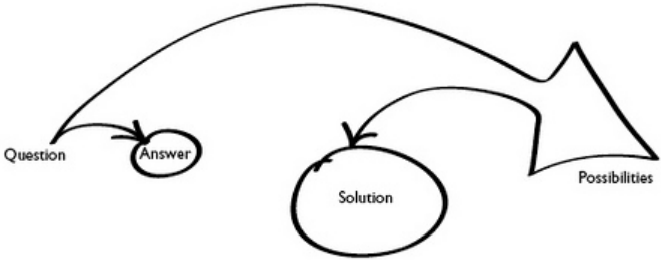
\includegraphics[width=\columnwidth]{figure1.png}
    \caption{Framework illustrating a linear problem solving approach versus a creative problem solving approach rooted in the design process. Once possibilities are explored, they can be scaled back and reconciled with reality to produce more effective and innovative solutions. }
\end{figure}

If Figure 1 is about the general arc of the process, Figure 2 is about interactions and reactions to others who are involved with the process. Figure 1 and Figure 2 both address bringing awareness to one’s approach in order to be more open to ideas and exploration early in the design process.

Figure 2 shows The Six Thinking Hats (De Bono, 1999), a useful framework for one’s mindset and interactions during the design process. All of these Thinking Hats are necessary. They are useful at different \textit{stages} of the design process and should be “worn” intentionally.

\begin{figure}[h!]
    \centering
    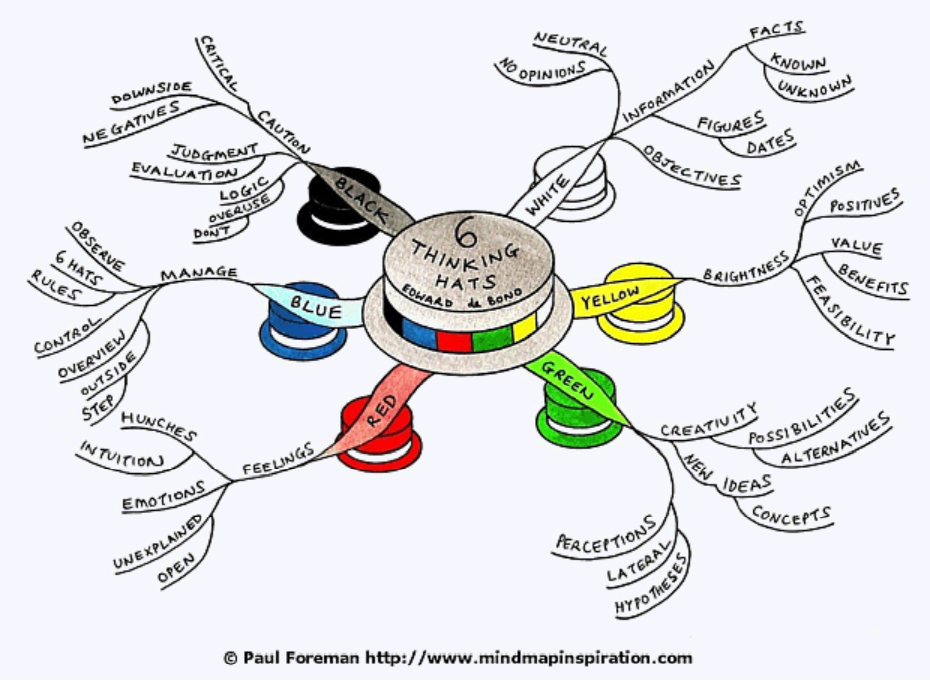
\includegraphics[width=\columnwidth]{figure2.png}
    \caption{Framework illustrating different types of interactions that people can have with one another. Different “hats” are beneficial during different stages of the design process. Awareness of this framework, and which hat is most beneficial when, can help create a collaborative and supportive atmosphere that cultivates creativity. (Foreman, 2020)}
\end{figure}

BLACK hats are commonly “worn” by linear thinkers. If “worn” during early ideation, BLACK hats will result in a linear problem solving approach. If a creative problem solving approach is desired, BLACK hats are counterproductive during this early phase. They are useful in later stages of the design process when ideas are being narrowed and refined. 

GREEN and YELLOW hats should be “worn” for generative ideation and brainstorming, particularly in the early ideation stages of the design process. This promotes open exploration of possibilities and encourages ideas to build off of one another.     

It is often helpful to have shared language to discuss what is happening at a given time during the design process. There are a number of design processes that exist and most are fairly comparable. Figure 3 shows the author’s design process that is used in BOOST Workshops. It consists of nine non-linear components that can occur simultaneously and repeat throughout the process.

\begin{figure}[h]
    \centering
    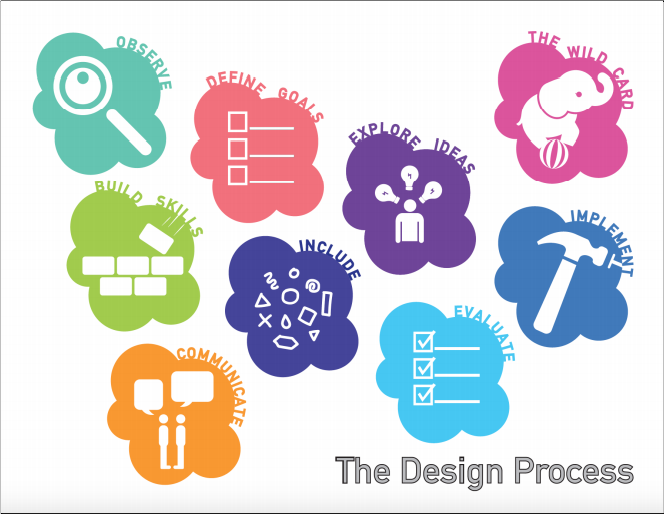
\includegraphics[width=8cm]{figure3.png}
    \caption{The BOOST Workshop design process contains nine non-linear components. These components can occur simultaneously and at multiple points during the process}
\end{figure}

\begin{itemize}
    \item 	Observe: Involves researching, mapping, measuring, interviewing and other methods to understand the context.
\item 	Define Goals: Determine what you are setting out to do. Define what the solution should \textit{do} rather than what it should \textit{be}. Define your goals and constraints.  
\item 	Build Skills: Learning a new tool or skill, or bringing in an expert might be necessary to realize your project. 
\item 	Explore Ideas: Go broad and wide with your brainstorming. Outlandish ideas are encouraged. 
\item 	Implement: Narrow and refine your idea(s). Create prototypes to test them. 
\item Include: If people with different demographics are expected to use this solution, bring other perspectives in to co-design \textit{with} you.
\item 	Communicate: Written and oral as much as visual and graphic. Describe the idea through multiple media to give a clearer picture of your vision. 
\item 	Evaluate: Revisit the goals and constraints that were defined to ensure the idea is successful. 
\item 	The Wild Card: The external world may have an unexpected impact on an idea or project. It can sometimes seem disastrous. Embrace the unexpected: revisit the goals, revise the constraints, and find a new path forward.        
\end{itemize}

\subsection*{Reframing the Mindset}

Our society has deeply ingrained biases against people with disabilities. These harmful mindsets are often ingrained and invisible to most people. Figure 4 challenges this common set of biases, and offers a different way of thinking that is more empowering for people with disabilities. 

\begin{table*}[th]
\caption*{Reframing the Question/Mindset for Empowerment}
\label{tab:my-table}
\begin{tabular}{|c|c|}
\hline
\textbf{Common Assumptions Around Disability} & \textbf{Consider, instead...} \\ \hline
A disability = a problem to be solved  & A disability = a lifelong condition, an identity to celebrate, a community to be a part of \\ \hline
Assistive devices look Medical / User looks like a "patient" &  \begin{tabular}[x]{@{}c@{}}Assistive devices look trendy and stylish (eg glasses) User looks dignified, independent, fashion-forward \\ Opportunity for self-expression \end{tabular} \\ \hline
People with disabilities (PWD) are in need of help / Recipients of aid &  PWD are capable of creating their own solutions, and know their needs best. \\ \hline
PWD understood to be "Need knowers" and "End users" & \begin{tabular}[x]{@{}c@{}} PWD seen as designers + makers \\ Designer who is also end user \end{tabular} \\
Missing or lacking something, disadvantaged & Whole just as they are. Unique perspective + capabilities such as creativity + adaptability \\ \hline
Assistive devices, prosthetics & Body mods, enhancement to the natural body (blur distinction between prosthetic + exoskeleton) \\ \hline
Assistive devices as functional, efficient & Assistive devices as expressive, beautiful, dignified \\ \hline
Focus on what a body lacks & Focus on what a body has  \\ \hline
Focus on body & Focus on experience  \\ \hline
\end{tabular}
\captionof{figure}{This table proposes a more empowered way of thinking about disability than the mindset that is common in American media and society.}
\end{table*}

\subsection*{Working with Able-Bodied Youth on Disability Challenges}

Many educators are inclined to bring this project type and approach into their K-12 classroom which does not include any or many youths with disabilities. This can be problematic and is not recommended for a few reasons. It can create a dynamic of designing FOR and not WITH. 
First, it can reinforce an imbalanced and disempowering dynamic, where the able-bodied youth are the “helpers” and the youth with a disability is the one being “helped.” Second, while the able-bodied youth might feel positive about the solution they create, it may be built on false assumptions and not actually be useful or desirable for its recipient. 
These challenges may be addressed. For example, able-bodied youth may begin by designing for themselves, based on their own needs. They may collaborate as equal partners with a youth with a disability, and perhaps even design solutions for each other (so the able-bodied youth receives a prototype from the youth with a disability, and vice-versa).  

\subsection*{Leading a Hands-On Design Workshop}

The aforementioned frameworks and methodologies can be successfully used with a broad range of demographics and project types. They are central to a design or creative problem solving approach.  
The following are recommendations for leading a hands-on design workshop:
\begin{itemize}
\item 	Start prototyping as soon as possible, rather than waiting for the perfect opportunity. Use paper and tape to create fast and easy prototypes. 
\item 	Spend time creating the right environment for generating ideas, which will be advantageous later in the project. 
\item 	Be mindful to design WITH not FOR. 
\item 	When working with people with disabilities, reframe the questions and mindset for empowerment.
\item 	Let go of assumptions and expectations. Let the youth drive their project ideas. 
\item 	Facilitators don’t need to have all of the answers. Figure it out together with the youth.
\end{itemize}

\subsection*{BOOST Workshops}

While a range of formats have been tested from pop-up public engagements to 5-day intensives, the most effective format has been found to be the 5-day intensive, which will be the focus of this section. Although this 5-day format is preferred, it is not always feasible. There are still lessons to be learned from it, and less intensive methods may be used.   

These workshops typically engage 6-10 participants ages 10-18, and attempt to maintain a 1:1 ratio of participants to facilitators. Participants have included youth with upper and lower limb differences, and wheelchair users, and they are recruited through support organizations and healthcare providers. While BOOST Workshops engage participants with physical disabilities, they were developed for youth with any level of ability. Rather than focus on deficits, they invite participants to create something to enhance their body, however their body is. 

By the end of the workshop, each participant has developed their own functional and completely unique prototype.  

Facilitators are generally design students pursuing an advanced degree or design professionals. Each facilitator is required to attend a facilitation training. A prosthetist attends portions of each workshop (on Days 3+4) to support participants in attaching their prototypes to their bodies safely and comfortably. 

Day 1 + Day 2 focus on creating the right environment, exploring ideas, and learning tools and technology. Tools and technologies taught have ranged from 3D scanning, modeling, and printing, to plaster casting, to sewing, to basic electronics. Days 3 + 4 are dedicated to developing ideas and building prototypes with the tools available. Participants generally work intensively with facilitators on these days on their individual projects. On Day 5, participants finalize their prototypes and give a public presentation on their work. This presentation is essential not only to serve as a hard deadline for prototype completion, but also as an opportunity to reflect on and celebrate participant’s work and inspire attendees. 

At the end of each workshop, participants may choose to be partnered with design and engineering professionals for 4-6 months to continue developing their prototype. These groups generally begin by establishing goals and expectations. They typically meet on a weekly basis to collaborate on the project. In these collaborations, the youth continues to drive the design vision, and the facilitator may challenge ideas or push them further, and support with the more technical production of the final prototype. These collaborations generally culminate in another final public presentation.   

\section*{IMPACT}

BOOST Workshops have significantly impacted individual participants' lives in terms of opening up new opportunities and career paths. Anaiss A. developed a wheelchair lift that raises her wheelchair two inches off the ground using two 3D printed stilts attached to her wheelchair. 
\begin{figure}[h]
    \centering
    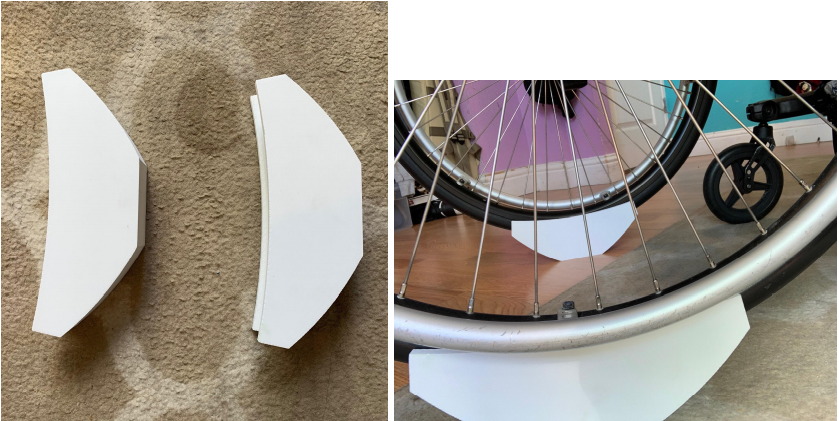
\includegraphics[width=8cm]{figure5.png}
    \caption{Images of Anaiss A.’s wheelchair lift, from the side view (left) and in use (right). These pieces fit snugly onto the wheels to safely roll up to and down from a 2” height. They have been likened to “tippy toes for your wheelchair.” (Courtesy of Anaiss A.) }
\end{figure}
Since attending a BOOST Workshop in 2018, Anaiss uses her wheelchair lift and is trying to find ways to share her invention with other wheelchair users. She has also written a Medium article on the relationship between disability and design and presented at multiple conferences such as ISLAND 2020 and the Nelson Atkins Museum. Anaiss plans to be a pediatrician in the rehabilitation division to be a role model to kids who, like her, experienced traumatic injuries that leave them paralyzed. The BOOST Workshops gave her more confidence in her disability and the work she can do. \textit{"Being surrounded by other participants with disabilities opened my eyes to the possibilities of my future careers. I didn't think about my dream jobs as blocked by obstacles. I only saw challenges I would overcome."}

Anaiss is not the only participant for whom this approach has opened new opportunities.The following youth participants were all born with an upper limb difference, and each designed a wearable device for themselves which led to additional opportunities beyond the BOOST workshop.
\begin{figure}[h]
    \centering
    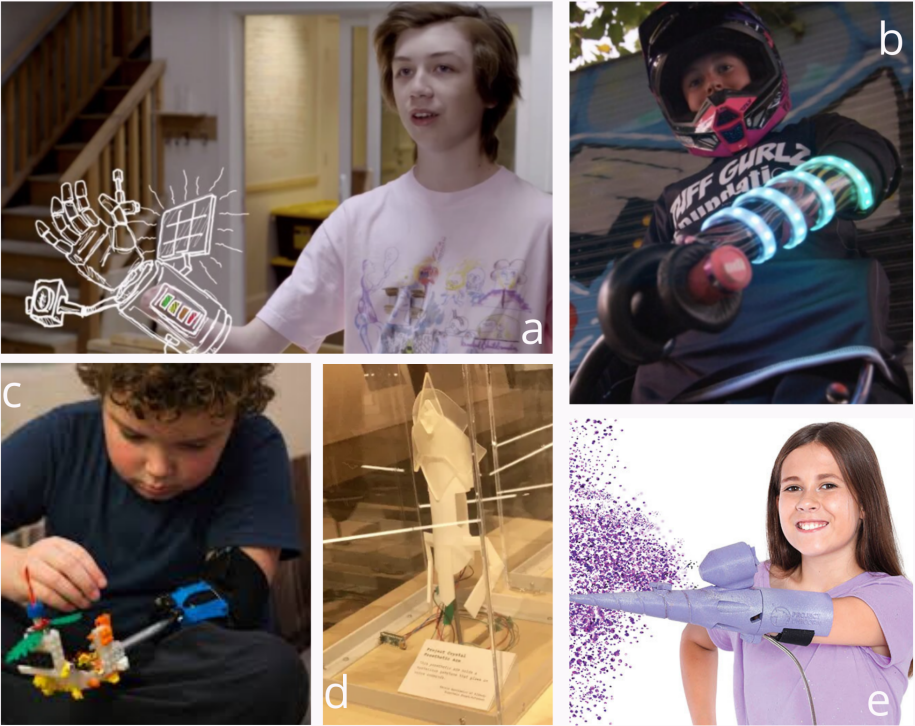
\includegraphics[width=8cm]{figure6.png}
    \caption{Previous BOOST Workshop participants with their design projects. (a)
Kieran C. and his creation “Nubinator 2.0,” (b) Sydney H. and her design for a BMX
bicycle prosthetic, (c) Aidan R. and his project, the “Superhero Arm,” (d) Kenzie W.’s
design for “Operation Crystal,” (e) Jordan R.’s creation, a glitter blaster called “Project
Unicorn”. }
\end{figure}
\begin{itemize}
    \item 	Kieran C.’s “Nubinator 2.0” (Figure 6a) is a 3D printed prosthetic arm with
atypical features such as a toy dart shooter and LED lights. Kieran’s
project - and his ideas for future iterations of his design - was featured on HistoryNOW (Kids, 2017), and he plans to become a digital fabrication
expert, with a focus on designing prosthetics.
\item 	Sydney H. (Figure 6b) was highlighted by Autodesk as a Tinkercad Hero
for her project (Autodesk, 2018), a BMX bicycle prosthetic enhanced with
color-changing LEDs, and she presented her work on a main stage at the
Bay Area Maker Faire in 2016.
\item 	Aidan R. created a “Superhero Arm” (Figure 6c), which has
interchangeable attachments such as a lego hand, violin bow, utensils,
and Nintendo Wii nunchucks for playing video games. Aidan presented his
work at the 2015 White House Maker Faire (Unger, 2015) and his
Superhero Arm was featured at the Design Museum Boston’s “Bespoke
Bodies” exhibit (Bespoke, 2019).
\item Kenzie W.’s “Operation Crystal” (Figure 6d), a voice-activated, illuminated,
sculptural wearable for her congenitally amputated arm, was exhibited at
the Chicago MSI’s “Wired to Wear” exhibit (Wired, 2019), and she is
currently pursuing toy design at Otis College. 
\item 	Jordan R. created “Project Unicorn” (Figure 6e), a 3D-printed glitter blaster
to wear on her congenitally amputated arm. Project Unicorn has since
launched her onto the national stage as a public speaker (Reeves, 2017),
author (Reeves, 2019), and disability rights advocate (Reeves).
\end{itemize}

The BOOST Workshops were not the end of participants’ learning careers, as some of them joined together to create a business that would bring a new perspective to industry professionals. 

A selected few BOOST alumni decided in 2019 to create an inclusive design consultancy to bridge the gap between the disability community and the design community. This firm is focused on providing access to industry professionals to design \textit{with} individuals with disabilities and not \textit{for} them. The goal of the consultancy is to amplify disabled voices and perspectives in the design process, shifting perceptions around inclusion and increasing visibility in society as a whole. It is challenging designers and engineers to design their products and services to be more inclusive. If successful, this will help to normalize disability and result in greater representation. 

Since its inception, this consultancy has published articles, spoken at conferences, participated in interviews and podcasts, and developed their own product ideas and design skills more deeply. It is building its expertise to provide consulting services to individuals and companies, inviting them to co-create with youth with disabilities throughout their process, rather than limiting disability involvement to user research and evaluations. This will allow people with disabilities to translate \textit{their own} lived experience into solutions, rather than designers translating on their behalf.  

\section*{DISCUSSION}

The BOOST approach to programming is rooted in a mindset of designing WITH, not FOR, as participants with disabilities are taught technical and design skills and supported in creating their own solutions. This approach exposes participants to careers in STEAM, which raises awareness about those career paths as students develop one-on-one relationships with professionals in those fields. STEAM careers - and more particularly, engineering and design - play a powerful role in shaping our world in a tangible way: they create the built environment we live in and the objects with which we interact. Not only are design outcomes improved when end users are incorporated into the process, but this approach has been shown to improve confidence in creating one’s own solutions. If individuals with disabilities see that STEAM skills and careers can directly affect their lives and the lives of others in a beneficial way, it will become a more diverse field with more practitioners from the disability community. This would result in increased inclusion in our society as a whole: those individuals will inherently develop more inclusive and accessible solutions in the mainstream that they themselves are able to use.   

The world is evolving and mindsets need to evolve too. Society has a history of telling people with disabilities that “they can’t” - in doing so, it strips away agency and views them as a burden. This must change and society needs to see people with disabilities differently. They must be viewed as people who can not only contribute, but who can offer unique insights and perspectives to drive meaningful and necessary societal change.

\section*{ACKNOWLEDGEMENTS}

Special thanks to Christine Ganim and Dara Rochlin for editing this article to make this publication possible, and to Born Just Right’s Board of Directors for its tireless support.

\end{large}
\clearpage
\section*{REFERENCES}\par 

\leftskip 0.25in
\parindent -0.25in 

Arreola, Anaiss N. “Design WITH Disability.” Nelson Atkins Museum of Art. 23 Nov. 2019, Nelson Atkins Museum of Art, Missouri.

Arreola, Anaiss N. “Disability Doesn't Destroy Design.” \textit{Medi\-um,} Medium, 18 Sept. 2019, \url{medium.com/@MakeJustRight/disability-doesnt-destroy-design-ede234f4e33.}

Autodesk Education. \textit{Student Maker: Sydney's Path from BMX to Tinkercad. Vimeo,} 26 Oct. 2018, \url{vimeo.com/297415556}.

“Bespoke Bodies.” \textit{Design Museum Everywhere,} 11 April 2019, \url{designmuseumfoundation.org/program/bespoke-bodies/}.

Cassim J. (2007) “‘It’s Not What You Do, It’s the Way That You Do It’: The Challenge Workshop - A Designer-Centred Inclusive Design Knowledge Transfer Mechanism for Different Contexts.” \textit{Universal Access in Human Computer Interaction: Coping with Diversity.} Lecture Notes in Computer Science, vol 4554. \url{https://doi.org/10.1007/978-3-540-73279-2\_5}

De Bono, Edward. (1999). \textit{Six Thinking Hats.} Penguin Books.

Dirth, Thomas P., and Nyla R. Branscombe. “SPSSI Journals.” \textit{Society for the Psychological Study of Social Issues,} John Wiley \& Sons, Ltd, 30 July 2019, \url{spssi.onlinelibrary.wiley.com/doi/abs/10.1111/josi.12345}

Foreman, P. (2020). “Six Thinking Hats Mind Map.” \textit{Mind Map Inspiration Art, Advice,  Encouragement,} Mind Map Inspired. \url{www.mindmapinspiration.com/six-think-ing-hats-mind-map-paul-foreman/.}

Ganim, Kate. \textit{Developing Trainings for Trainers.} Retrieved June 22, 2021 from \url{www.kateganim.com/work/train-ingtrainers.}\\

Hahn HD, Belt TL. Disability identity and attitudes toward cure in a sample of disabled activists. J Health Soc Behav. 2004 Dec;45(4):453-64. doi: 10.1177/00221465-0404500407. PMID: 15869116.

Heylighen, Ann, and Matteo Bianchin. “How Does Inclusive Design Relate to Good Design? Designing as a Deliberative Enterprise.” \textit{Design Studies,} Elsevier, 14 July 2012, \url{www.sciencedirect.com/science/article/abs/pii/S0142694X12000348.}

Holmes, Kat. (2020). Mismatch. The MIT Press. 

“Kids and Engineers Are Workshopping Superhero Cyborgs.” \textit{History.com,} A\&E Television Networks, 4 Oct. 2017, \url{play.history.com/shows/history-now/videos/kids-and-engineers-are-workshopping-superhero-cyborgs?playlist\_slug=history-now-science-and-technology.}

Luck, Rachael. “Inclusive Design and Making in Practice: Bringing Bodily Experience into Closer Contact with Making.” \textit{Design Studies,} Elsevier, 6 Dec. 2017, \url{www.sciencedirect.com/science/article/pii/S0142694X1730087X?via\%3Dihub.}

Make Just Right. \textit{Our POV.} Retrieved April 26, 2021 from \url{www.makejustright.com/pov.}

Petrides, Lisa, et al. (2020). “Action Collabs.” \textit{Action Collabs | Institute for the Study of Knowledge Management in Education.} \url{www.iskme.org/services/action-collabs.} 

Pullin, Graham. (2011). \textit{Design Meets Disability.} MIT Press. 

Reeves, Jordan. \textit{Born Just Right.} Aladdin Books, 2019.

Reeves, Jordan. \textit{Home Page.} Retrieved April 26, 2021 from \url{jordanreeves.com.}

Reeves, Jordan. “What Is Normal?” TEDxCoMo. 13 April 2017, The Missouri Theater, Missouri. \url{www.youtube.com/watch?v=5t7kFRQ5S-4.}

Srivastava, Pankaj. “The Power Of Yes: Why The Yes Mindset Leads To Innovation And Creates Great Leaders.” \textit{Forbes,} 17 May 2021, 
\url{www.forbes.com/sites/forbesbus-inesscouncil/2021/05/17/the-power-of-yes-why-theyes-mindset-leads-to-innovation-and-creates-great-leaders/?sh=f84cd4475400.}

Unger, Coby. \textit{Aidan's Superhero Arm at the White House. Vimeo,} 20 June, 2015, \url{vimeo.com/131316250}.

“Wired to Wear.” \textit{Museum of Science and Industry,} 21 March, 2019, \url{www.msichicago.org/explore/whats-here/exhibits/wired-to-wear/}.

\end{document}